\chapter{弱相互作用、维里修正与非恰当微分}

\lectureoverview{我们首先讨论测量与温度的操作性含义，然后追问当短程相互作用被微弱地开启时，稀薄气体如何偏离理想气体定律。配分函数给出能量与压强的首批相互作用修正，并确定其适用范围。最后的数学插曲借助恰当微分、闭合回路以及一个具体的理想气体检验，把态函数与路径依赖的热和功区分开来。}

\section{仪器实际测量的是什么}

没有任何实验室装置能直接伸入自然之中并报告一个抽象的数学变量。弹簧秤报告的是伸长量；温度计报告的是液柱高度。我们之所以把前者称为力的测量、把后者称为温度的测量，只是因为已经在可见响应与所需量之间建立起了一种可重复的关系。

这种关系有其有限的适用范围。弹簧只有在保持弹性时才服从胡克定律，而足够大的力最终会使其变形或断裂。更一般地，若一个光滑的读数\(R\)依赖于物理变量\(X\)，则在选定的工作点附近有
\begin{equation}
 \Delta R \simeq
 \left.\frac{dR}{dX}\right|_{X_0}\Delta X.
 \label{eq:sm6-local-linear-response}
\end{equation}
即使完整的响应曲线是非线性的，读数的小变化也与目标变量的小变化成正比。这种局部线性化正是校准的通常逻辑。

读数还可能依赖于干扰变量。弹簧可能对温度或压强有微弱的响应。温度计中水银柱的高度可能通过重力而随取向变化，也可能受玻璃性质或材料缓慢变化的影响。测量方案并不证明这些依赖关系不存在；它只是把它们固定住，或表明它们在所需尺度上可以忽略。

\begin{classroomqa}
\audiencequestion{局部引力场，或者温度计被拿持的方向，会不会改变读数？}
\lecturerresponse{原则上会。如果取向有可观的影响，那么竖直拿持温度计这一指令就成为该仪器定义的一部分。在地球表面附近，引力场足够稳定，剩余的变化通常可以忽略。
\lecturetimestamp{00:04:08--00:05:00}}
\end{classroomqa}

\begin{classroomqa}
\audiencequestion{老化或化学变化会不会缓慢地改变校准？}
\lecturerresponse{有可能。对于普通测量而言，水银和玻璃足够惰性，而在极其漫长的时间尺度上的变化与实验无关。校准始终是关于指定仪器、范围、方案和持续时间的陈述。
\lecturetimestamp{00:05:03--00:06:11}}
\end{classroomqa}

对于摄氏温度计，两个可重复的参考状态提供了一个方便的标度。若\(h_f\)和\(h_b\)分别是水在凝固点和沸点时的液柱高度，则在响应近似线性的范围内有
\begin{equation}
 T_{\mathrm C}=100\,\frac{h-h_f}{h_b-h_f}.
 \label{eq:sm6-celsius-calibration}
\end{equation}
在凝固点取\(T_{\mathrm C}=0\)是一种约定。它并不是热能为零的状态，正如冬日里华氏零度并非绝对零度。

\begin{figure}[t]
\centering

\includegraphics[width=0.90\textwidth]{lecture_06_figure_03.png}
\caption{一个光滑但非线性的温度计响应，其中标出了一段短区间用于线性校准。}
\lectureframe{00:07:55}
\end{figure}

\section{平衡与作为能量标度的温度}

只有当温度计与附近介质达到热平衡之后，温度计测量的才是其环境的温度。在此之前，它的读数只是在朝着平衡变化。实用的检验很简单：等到读数不再变化为止。这条规则的简单性掩盖了决定等待时间的那些物理过程。

\begin{classroomqa}
\audiencequestion{达到平衡是否只涉及球泡周围的一层边界层，又应当等待多久？}
\lecturerresponse{能量必须穿过玻璃并与周围介质交换，因此时间取决于温度计、其热导率以及介质。紧邻的环境还必须能代表一个均匀的平衡态。在实验上，当读数不再漂移时，就认为可以接受。
\lecturetimestamp{00:08:45--00:10:13}}
\end{classroomqa}

在这一等待时间中，温度与密度扮演着不同的角色。非常稀薄的气体可以非常热：其中为数不多的分子可能带有很大的动能。然而这些分子很少撞击温度计，因此达到平衡可能很慢。在保持温度不变的情况下把密度降低一百倍或一千倍，并不会降低分子的能量标度；它降低的是该能量被传递给仪器的速率。

\begin{classroomqa}
\audiencequestion{房间里的辐射温度可以不同于空气的温度吗？}
\lecturerresponse{可以。物质与辐射只有在彼此处于热平衡时才共享同一个温度。中性空气与照明房间中大部分光学辐射的耦合很弱，因此光子布居不必是处于空气温度下的平衡黑体场。
\lecturetimestamp{00:11:26--00:12:20}}
\end{classroomqa}

一旦建立平衡，温度最好被视为一种能量标度。我们继续使用\(k_B=1\)的单位制，因此\(T\)本身具有能量的量纲。对于单原子理想气体，
\begin{equation}
 E_0=\frac{3}{2}NT.
 \label{eq:sm6-ideal-energy}
\end{equation}
每个分子的热能由\(T\)固定；相应的速率仍然依赖于分子质量。

\section{开启弱相互作用}

\begin{classroomqa}
\audiencequestion{在什么条件下理想气体近似会失效，并且这种失效能否用数学方式展示？}
\lecturerresponse{从已求解的非相互作用气体出发，开启一个小的相互作用。按该变化量展开，计算第一阶修正，并将其与理想项比较。当修正不再小时，该近似失效。
\lecturetimestamp{00:12:25--00:14:40}}
\end{classroomqa}

这是标准的微扰策略。如果一个问题在\(\lambda=0\)时可解，就引入耦合\(\lambda\)，写出
\begin{equation}
 F(\lambda)=F(0)+\lambda F_1+\lambda^2F_2+\cdots,
 \label{eq:sm6-perturbative-template}
\end{equation}
并追问所保留的每一项是否都小于前一项。这里的参考问题是理想气体。物理上的小量来自稀薄的样品、比平均间距短的相互作用程，以及足够弱、使第一阶相互作用项有用的势。高密度或长程力可能使该近似失效，即使任何一次相遇看起来都很温和。

设\(x_i\in\mathbb R^3\)和\(p_i\in\mathbb R^3\)分别为分子\(i\)的位置和动量。对于质量为\(m\)的全同分子，取
\begin{equation}
 H(X,P)=
 \sum_{i=1}^{N}\frac{p_i^2}{2m}
 +\sum_{i<j}u\!\left(|x_i-x_j|\right),
 \label{eq:sm6-interacting-hamiltonian}
\end{equation}
其中\(X=(x_1,\ldots,x_N)\)，\(P=(p_1,\ldots,p_N)\)。限制条件\(i<j\)排除了自身配对，并且只将\((i,j)\)计数一次：
\begin{equation}
 \sum_{i<j}1=\binom{N}{2}=\frac{N(N-1)}{2}.
 \label{eq:sm6-pair-count}
\end{equation}

\begin{classroomqa}
\audiencequestion{为什么不分别对两个粒子标签独立求和？}
\lecturerresponse{对\((3,7)\)与对\((7,3)\)是同一个物理对，而且粒子不会与自身配对。将求和限制在\(i<j\)同时强制了这两个事实。质量符号保留为\(m\)，而\(i,j\)用于标记粒子，以避免当\(m\)被同时用于这两种用途时可能出现的记号冲突。
\lecturetimestamp{00:17:52--00:19:12}}
\end{classroomqa}

将总构型势写为
\begin{equation}
 U(X)=\sum_{i<j}u\!\left(|x_i-x_j|\right).
 \label{eq:sm6-total-potential}
\end{equation}
假定相互作用具有平移不变性且为短程：当\(r\)与分子长度相比很大时，\(u(r)\)变得可忽略。

\section{积分后的对强度}

只有弱对势的一个积分进入第一阶修正：
\begin{equation}
 U_0\equiv\int_{\mathbb R^3}d^3r\,u(r).
 \label{eq:sm6-u0-definition}
\end{equation}
其单位是能量乘以体积。它把相互作用的典型强度与该相互作用可观的体积结合起来。

\begin{figure}[t]
\centering
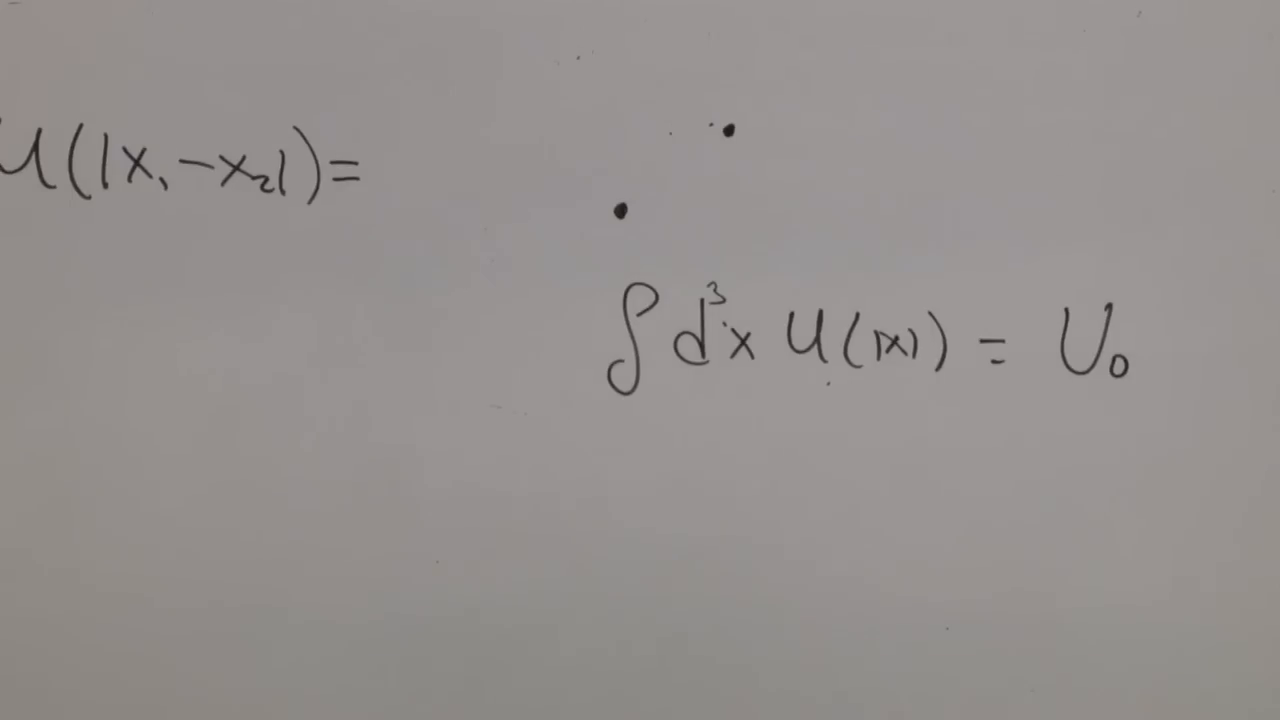
\includegraphics[width=0.90\textwidth]{lecture_06_figure_04.png}
\caption{短程对势被压缩为积分强度\(U_0=\int d^3r\,u(r)\)。}
\lectureframe{00:25:15}
\end{figure}

为了看清\(U_0\)为何有用，考虑一个对：
\begin{equation}
 I_2=\int_V d^3x_1\,d^3x_2\,
 u\!\left(|x_1-x_2|\right).
 \label{eq:sm6-two-particle-integral}
\end{equation}
引入相对坐标\(r=x_2-x_1\)。远离边界时，相对积分给出\(U_0\)，而该对的共同位置则遍历整个容器。因此
\begin{equation}
 I_2=V U_0+\text{surface corrections}.
 \label{eq:sm6-pair-integral-vu0}
\end{equation}
修正来自距壁面一个相互作用程内的粒子，此时相对坐标邻域的一部分位于盒子之外。其相对重要性按表面积与体积之比标度，并在宏观极限下消失。

\begin{classroomqa}
\audiencequestion{\(U_0\)指的是某个选定的对，并且是否让一个粒子与另一个粒子保持固定间距？}
\lecturerresponse{它指的是任意一个对所遵循的共同相互作用规律。将第一个粒子固定，对第二个粒子的所有相对位置积分。在此积分过程中间距并不固定。只有附近的相互作用区域有可观贡献，从而产生\(U_0\)。
\lecturetimestamp{00:26:03--00:27:33}}
\end{classroomqa}

\begin{classroomqa}
\audiencequestion{为什么第二个位置积分给出整个容器的体积，而第一个不给出？}
\lecturerresponse{在相对构型被积分成\(U_0\)之后，整个对可以在样品中平移。这种共同平移提供了大因子\(V\)。相互作用邻域是一个分子尺度的体积，已经包含在\(U_0\)之内，而不是另一个等于容器体积的因子。
\lecturetimestamp{00:27:48--00:29:21}}
\end{classroomqa}

\begin{classroomqa}
\audiencequestion{这个值会不会依赖于固定的是哪个点，尤其是在壁面附近？}
\lecturerresponse{平移不变性使得体相值与固定点无关。在壁面附近，积分会略有不同，因为有些邻近位置不可用。只有分子厚度的表面层受到影响，因此当盒子是宏观尺度时，误差可以忽略。
\lecturetimestamp{00:29:24--00:31:22}}
\end{classroomqa}

\begin{classroomqa}
\audiencequestion{结果是不是对每一个两粒子构型积分后的势能，为什么它只正比于一个大的体积？}
\lecturerresponse{是的。它的单位是能量乘以体积的平方，因为\(V U_0\)包含一个容器体积和一个分子相互作用体积。其中只有前者随样品尺寸增大。
\lecturetimestamp{00:31:31--00:32:04}}
\end{classroomqa}

\begin{classroomqa}
\audiencequestion{选择在固定体积下面积最小的球，会改变体相答案吗？}
\lecturerresponse{它只改变很小的边界修正。对于任何普通的宏观形状，距表面一个分子距离内的粒子数与体相中的粒子数相比可以忽略。只有当容器本身接近分子尺度时，表面才变得重要。
\lecturetimestamp{00:32:04--00:33:58}}
\end{classroomqa}

\begin{classroomqa}
\audiencequestion{用势代替粒子轨迹，是否就把碰撞省略掉了？}
\lecturerresponse{没有。力是势的导数，正是它产生碰撞。平衡态统计力学并不要求我们逐一追踪这些碰撞；它们的效果被编码在能量中，因而也编码在玻尔兹曼权重中。
\lecturetimestamp{00:33:59--00:35:29}}
\end{classroomqa}

\begin{classroomqa}
\audiencequestion{保留对力而不保留真正的三体相互作用，会损失什么？}
\lecturerresponse{微观能量可以包含真正的三体项，而对势的高阶项也会产生多粒子关联。然而在稀薄气体中，指定的三个粒子占据同一个分子邻域的可能性远小于两个粒子。因此对效应给出第一阶密度修正；更高的集团项以更高阶的密度幂次进入。
\lecturetimestamp{00:35:29--00:38:14}}
\end{classroomqa}

\section{自动运行下的配分函数}

统计方法的优势现在显现出来了。一旦哈密顿量给定，就无需猜测壁面附近或碰撞过程中的详细速度分布。我们写出正则配分函数并遵循其代数运算：
\begin{equation}
\begin{aligned}
 Z&=
 \frac{1}{N!h^{3N}}
 \int d^{3N}P\,d^{3N}X\\
 &\qquad{}\times e^{-\beta K(P)}e^{-\beta U(X)},\\
 K(P)&=\sum_i\frac{p_i^2}{2m}.
\end{aligned}
 \label{eq:sm6-full-partition-function}
\end{equation}
因子\(h^{3N}\)使经典相空间测度无量纲化，而\(N!\)消除了全同粒子的置换重复计数。

\begin{figure}[t]
\centering
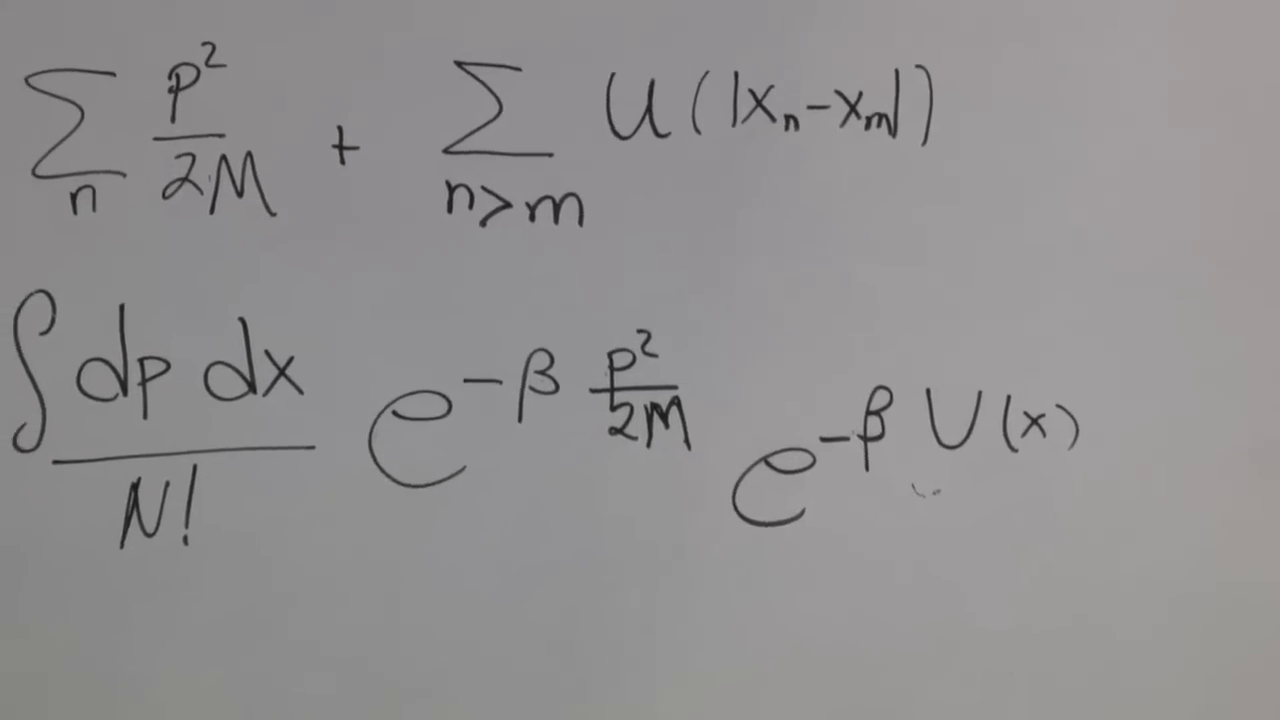
\includegraphics[width=0.90\textwidth]{lecture_06_figure_05.png}
\caption{多粒子能量以及配分函数中相应的动能因子和构型因子。}
\lectureframe{00:40:35}
\end{figure}

动量与位置分离。将构型积分乘以并除以\(V^N\)，即可分离出理想气体结果：
\begin{align}
 Z
 &=\left[
 \frac{V^N}{N!h^{3N}}
 \int d^{3N}P\,e^{-\beta K(P)}
 \right] \notag\\
 &\quad\times\left[
 \frac{1}{V^N}
 \int d^{3N}X\,e^{-\beta U(X)}
 \right] \notag\\
 &\equiv Z_0\,C(\beta,V,N).
 \label{eq:sm6-z-factorization}
\end{align}
熟悉的高斯因子为
\begin{equation}
 \int d^{3N}P\,e^{-\beta K(P)}
 =\left(\frac{2\pi m}{\beta}\right)^{3N/2}.
 \label{eq:sm6-gaussian-factor}
\end{equation}

\begin{figure}[t]
\centering
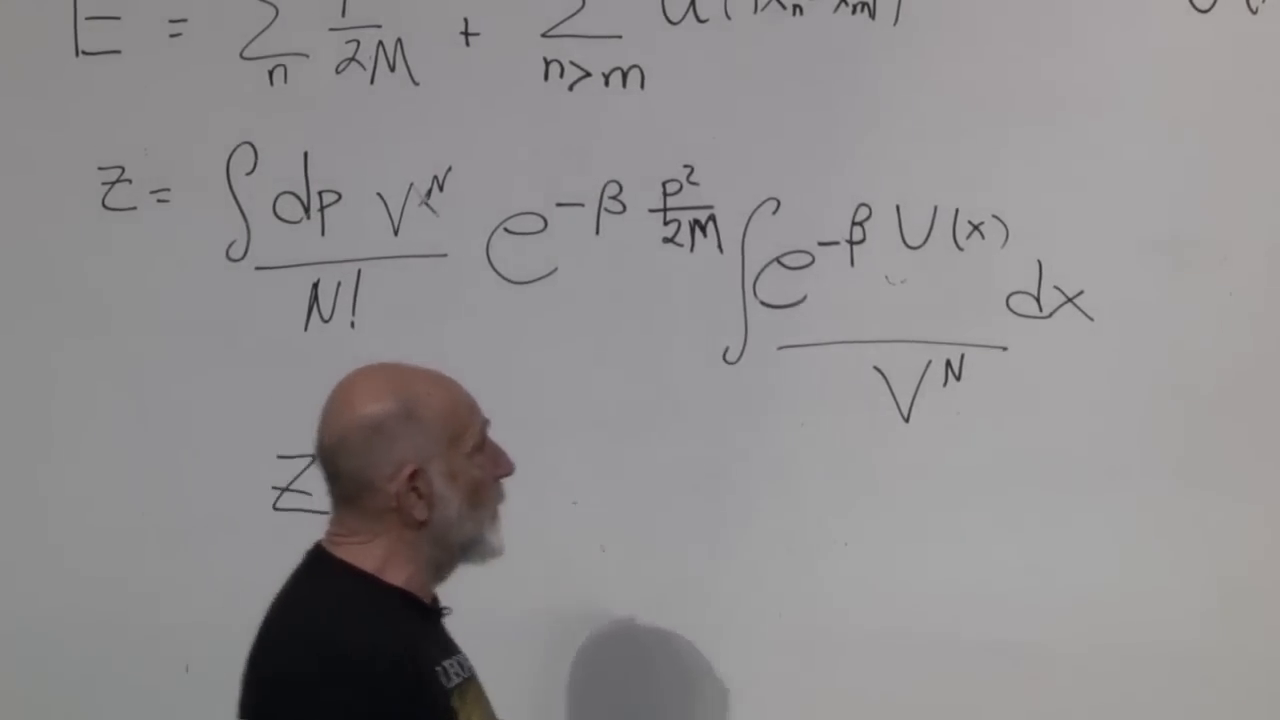
\includegraphics[width=0.90\textwidth]{lecture_06_figure_06.png}
\caption{从归一化构型因子中分离出的理想气体配分函数。}
\lectureframe{00:43:45}
\end{figure}

因子\(N!\)不影响归一化比值\(C\)，也不影响下文所用的特定固定\(N\)导数，但它并非可以从整体热力学中省略：它对于正确的状态计数和广延熵是必不可少的。

到相互作用的一阶，
\begin{equation}
 e^{-\beta U(X)}
 =1-\beta U(X)+O(U^2).
 \label{eq:sm6-boltzmann-expansion}
\end{equation}
因此，
\begin{align}
 C
 &=
 1-\frac{\beta}{V^N}
 \sum_{i<j}
 \int d^{3N}X\,u(|x_i-x_j|)
 +O(U^2) \notag\\
 &=
 1-\frac{\beta}{V^N}
 \frac{N(N-1)}{2}
 V^{N-2}(V U_0)+O(U^2) \notag\\
 &=
 1-\beta\frac{N(N-1)}{2V}U_0+O(U^2).
 \label{eq:sm6-configurational-correction}
\end{align}
每一对都有相同的\emph{积分}，而不是相同的瞬时间距或势能。剩余的\(N-2\)个位置积分各贡献一个\(V\)因子。

\begin{figure}[t]
\centering
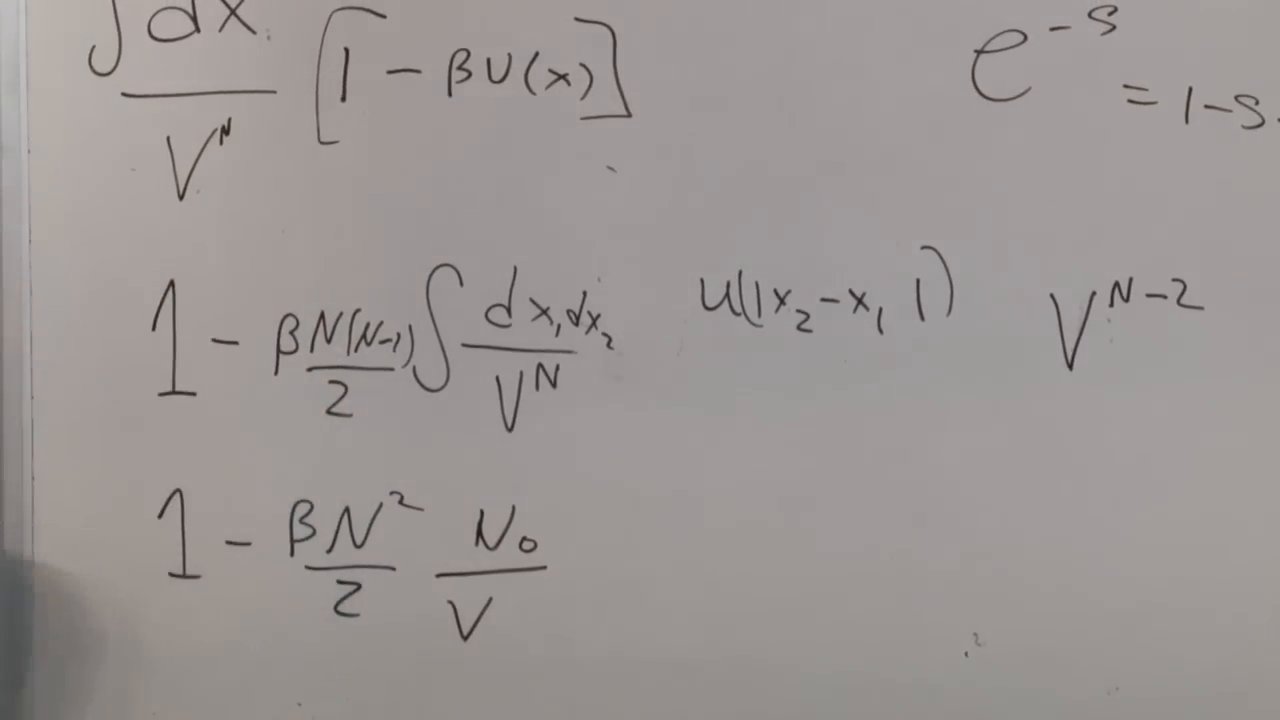
\includegraphics[width=0.90\textwidth]{lecture_06_figure_07.png}
\caption{对计数、旁观者坐标体积以及第一阶构型修正\(1-\beta N^2U_0/(2V)\)。}
\lectureframe{00:53:40}
\end{figure}

\begin{classroomqa}
\audiencequestion{领头项\(1\)是否假设势在零间距处为零？}
\lecturerresponse{不是。它是指数级数中的零阶项，与\(u(0)\)的值无关。势出现在下一项\(-\beta U(X)\)中。
\lecturetimestamp{00:46:19--00:46:48}}
\end{classroomqa}

\begin{classroomqa}
\audiencequestion{如果不同的对有不同的间距，为什么每一对都可以用同一个表达式代替？}
\lecturerresponse{并不是把它们的逐点值等同起来。每一项都在同一个完整构型空间上积分，而粒子标签并不区分这一对和那一对。这些积分具有相同的形式和相同的值。
\lecturetimestamp{00:50:00--00:51:07}}
\end{classroomqa}

\begin{classroomqa}
\audiencequestion{配对数究竟是\(N(N-1)/2\)还是
\(N(N+1)/2\)？}
\lecturerresponse{是\(N(N-1)/2\)：选定一个粒子后，只有\(N-1\)个不同的伙伴，而除以二则去除了反向的排序。对于宏观的\(N\)，将\(N(N-1)\)替换为\(N^2\)只改变一个相对的\(1/N\)修正。
\lecturetimestamp{00:48:33--00:49:56}}
\end{classroomqa}

由于\(\log(1-x)=-x-x^2/2-x^3/3-\cdots\)不是交错级数，一阶对数项为
\begin{equation}
 \log Z
 =
 \log Z_0
 -\beta\frac{N(N-1)}{2V}U_0
 +O(U^2).
 \label{eq:sm6-logz-correction}
\end{equation}
在\(N\)很大时，我们可以将\(N(N-1)\)替换为\(N^2\)，此时不需要有限\(N\)的区分。

\begin{remark}
受控的低密度表述使用Mayer函数
\(f(r)=e^{-\beta u(r)}-1\)以及第二维里系数
\begin{equation}
 B_2(T)=-\frac{1}{2}\int d^3r\,f(r).
 \label{eq:sm6-second-virial}
\end{equation}
对于弱势，\(f(r)\simeq-\beta u(r)\)，因此
\(B_2\simeq\beta U_0/2\)，从而重新得到下面的结果。对于硬排斥核心，这一形式是必需的，因为直接展开\(e^{-\beta u}\)并不成立。
\end{remark}

\section{能量、压强以及修正的含义}

\(Z\)的对数之所以有用，是因为它的导数是可以测量的。假设微观势与温度无关，
\begin{align}
 E
 &=-\left(\frac{\partial\log Z}{\partial\beta}\right)_{V,N} \notag\\
 &=
 \frac{3}{2}NT
 +\frac{N(N-1)}{2V}U_0+O(U^2) \notag\\
 &\simeq
 N\left(\frac{3}{2}T+\frac{1}{2}\rho U_0\right),
 \qquad
 \rho=\frac{N}{V}.
 \label{eq:sm6-energy-correction}
\end{align}
表面上非广延的\(N^2\)伴随着\(1/V\)。在固定密度下，\(N^2/V=N\rho\)，因此总能量仍然与系统的尺度成正比。每个粒子的额外能量与密度成正比，因为一个被选定的分子只有在另一个分子位于附近时才会获得对能量。

\begin{figure}[t]
\centering
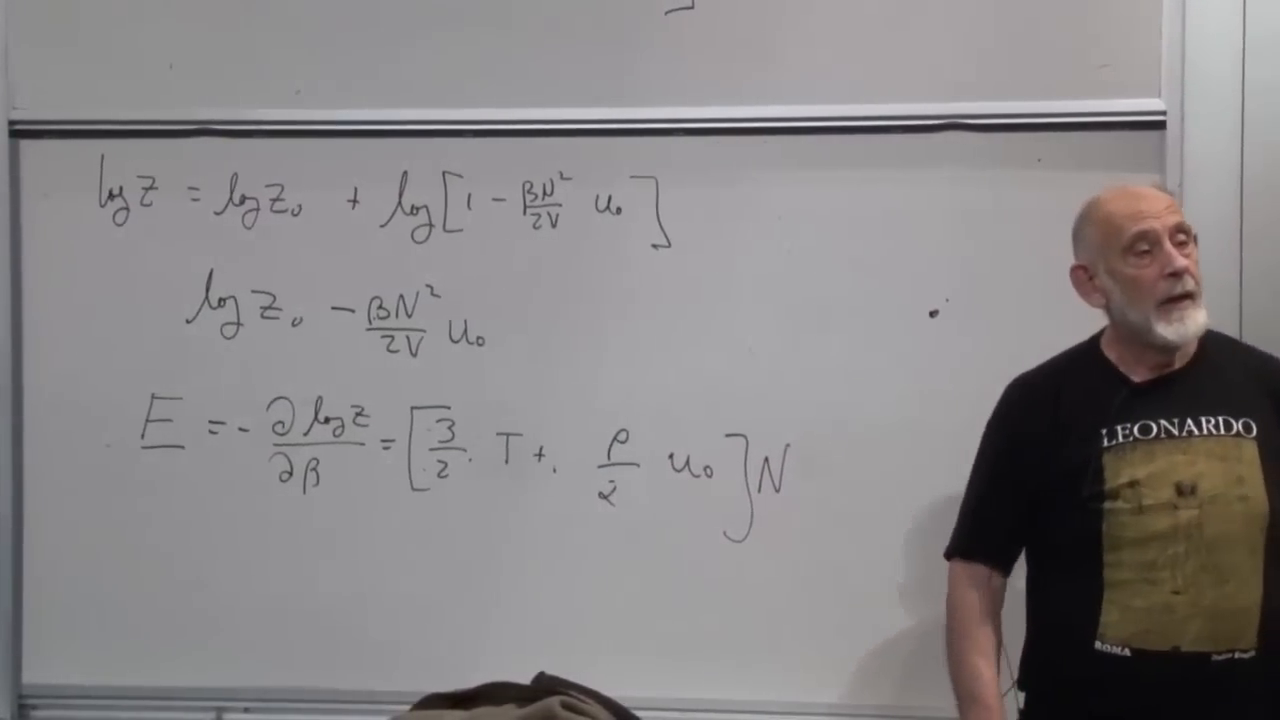
\includegraphics[width=0.90\textwidth]{lecture_06_figure_08.png}
\caption{第一项相互作用修正被重新组织为广延能量\(N[3T/2+\rho U_0/2]\)。}
\lectureframe{01:03:25}
\end{figure}

压强更容易测量。利用上一章的结果，
\begin{equation}
 P=T\left(\frac{\partial\log Z}{\partial V}\right)_{T,N},
 \label{eq:sm6-pressure-from-z}
\end{equation}
我们得到
\begin{align}
 P
 &=
 \frac{NT}{V}
 +T\frac{\partial}{\partial V}
 \left(-\beta\frac{N(N-1)}{2V}U_0\right)
 +O(U^2) \notag\\
 &=
 \rho T+\frac{1}{2}\rho^2U_0
 +O\!\left(\frac{\rho U_0}{N},U^2\right).
 \label{eq:sm6-pressure-correction}
\end{align}

\begin{figure}[t]
\centering
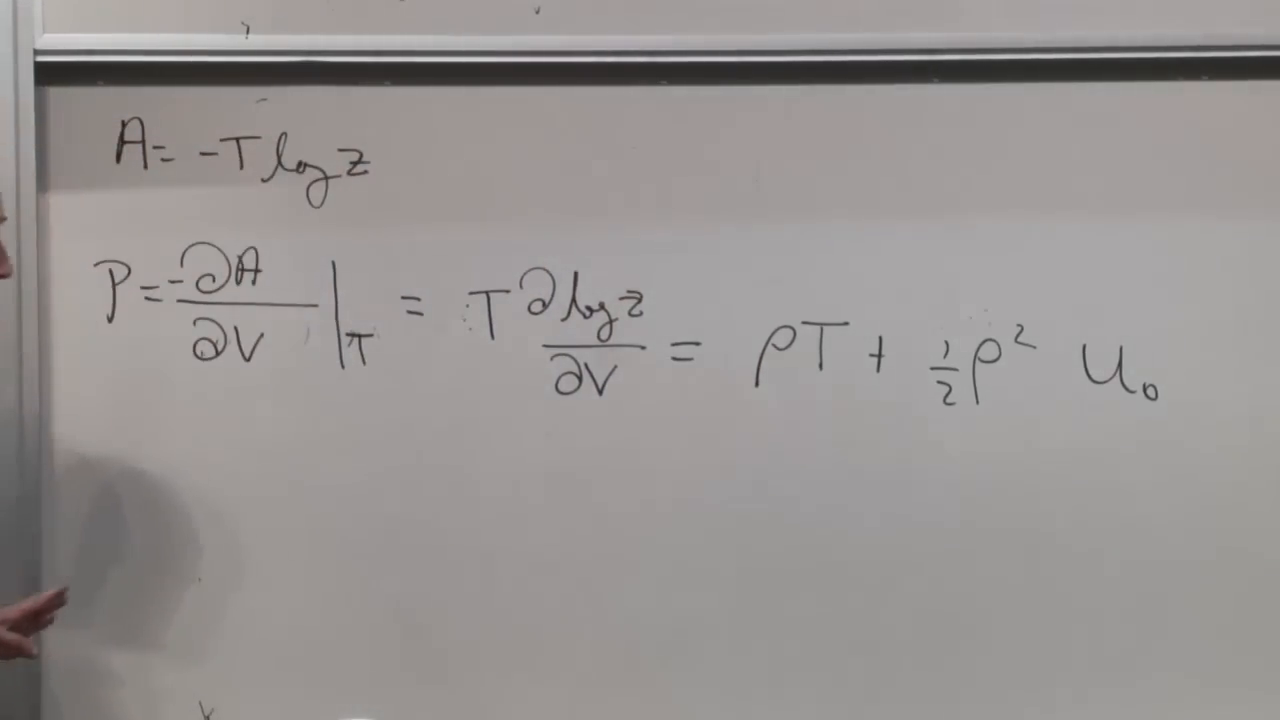
\includegraphics[width=0.90\textwidth]{lecture_06_figure_09.png}
\caption{由Helmholtz导数得到的压强，包含第一个二次密度修正。}
\lectureframe{01:09:50}
\end{figure}

\begin{classroomqa}
\audiencequestion{为什么\(\rho^2\)，而不是另一个幂次，才是自然的第一项修正？}
\lecturerresponse{理想项要求有一个粒子出现在一个小区域内，因此按\(\rho\)标度。相互作用则要求有两个粒子占据同一个分子邻域，其概率按\(\rho^2\)标度。因子\(1/2\)正是那个配对计数因子，它防止\((i,j)\)和\((j,i)\)被分别计数。
\lecturetimestamp{01:24:27--01:26:00}}
\end{classroomqa}

在固定温度下，可以改变\(V\)，测量\(\rho=N/V\)，并绘制压强。理想定律是线性项。\(P(\rho)\)的曲率揭示了第一项相互作用修正。在这个弱势近似内，该修正没有显式的温度依赖，因为\eqref{eq:sm6-pressure-from-z}中的因子\(T\)与\(\beta=1/T\)相消。

\begin{classroomqa}
\audiencequestion{密度可以增大到多大，才必须包含三体效应？}
\lecturerresponse{密度计数表明，下一个维里项与\(\rho^3\)成正比，但仅凭\(U_0\)无法推断其系数。它来自对相互作用的关联乘积的贡献，以及如果存在的话，真正的三体力。必须计算下一个集团系数，并将其与\(\rho^2\)项比较；不应把猜测的公式提升为结果。
\lecturetimestamp{01:10:50--01:13:38}}
\end{classroomqa}

当修正的幅度很小时，理想气体项占主导：
\begin{equation}
 \begin{aligned}
 \frac{1}{2}\rho^2|U_0|&\ll \rho T,\\
 |\rho U_0|&\ll T
 \qquad\text{(parametrically)}.
 \end{aligned}
 \label{eq:sm6-ideal-validity}
\end{equation}
第二个不等式的两边都是能量。量\(\rho U_0\)是每个粒子的相互作用能量尺度，而\(T\)是动能尺度。普通的稀薄室温气体远处于这一区域内；只有当分子邻域被占据得足够频繁，使相互作用足以与热运动相竞争时，才会出现显著的偏离。

\begin{classroomqa}
\audiencequestion{这个判据能对房间里的空气进行估计吗？}
\lecturerresponse{将\(U_0\)估计为分子相互作用能乘以分子体积，再乘以数密度，并将结果与\(k_BT\)比较。粗略的分子数值表明，在普通室内空气中相互作用尺度要小得多。需要相当大的压缩，分子才会频繁地挤入彼此的相互作用范围。
\lecturetimestamp{01:16:24--01:18:54}}
\end{classroomqa}

\begin{classroomqa}
\audiencequestion{\(U_0\)可以取两种符号吗？}
\lecturerresponse{可以。正的积分相互作用在这个近似中是净排斥的，并使压强高于\(\rho T\)。负的则是净吸引的，并使其降低。这个符号检验是对\eqref{eq:sm6-pressure-correction}的一个直接的物理检查。
\lecturetimestamp{01:18:56--01:20:29}}
\end{classroomqa}

\begin{figure}[t]
\centering
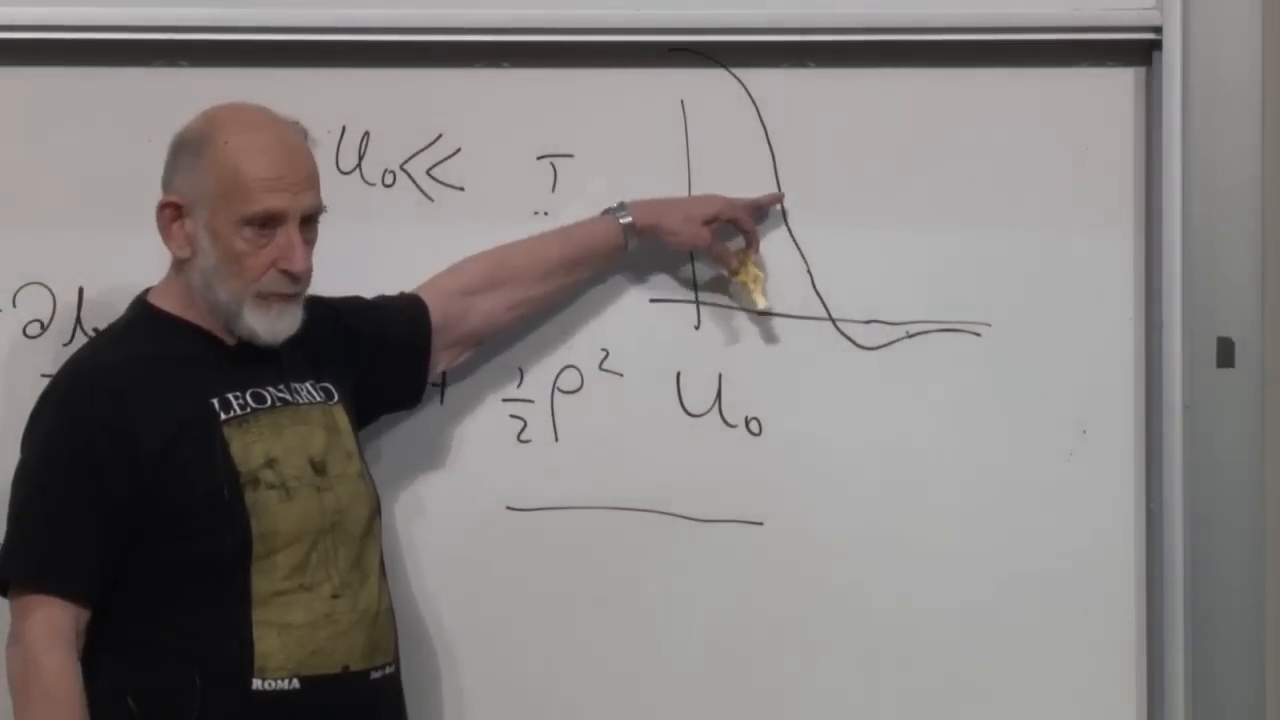
\includegraphics[width=0.90\textwidth]{lecture_06_figure_10.png}
\caption{定性的排斥和吸引对势曲线，旁边是压强公式，其修正跟随\(U_0\)的符号。}
\lectureframe{01:21:30}
\end{figure}

\begin{classroomqa}
\audiencequestion{静电斥力、引力或真实的分子力能否被纳入这一计算？}
\lecturerresponse{微观势来自原子物理、分子物理或量子物理的输入。中性分子通常表现出陡峭的短程排斥核心和较长的吸引性范德瓦尔斯尾部，常以12--6势示意性地表示。对于这样的硬核，应使用完整的Mayer函数公式。引力则不同：它是长程的，其空间积分不以所需的方式收敛，此处所用的通常短程热力学极限失效。
\lecturetimestamp{01:20:40--01:23:03}}
\end{classroomqa}

这一计算体现了一种有用的分工。微观物理提供\(u(r)\)。统计力学将该能量转化为\(Z\)，\(Z\)的导数给出宏观可观测量，而物理推理则检验其符号、密度标度、广延性和适用范围。只有在正确的能量和近似被选定之后，形式操作才是机械性的。

\section{恰当微分与路径依赖性}

现在我们更换数学语言。在\emph{恰当微分}这一说法中，恰当并不意味着数值上精确。它指的是一个一次形式是某个真正的标量函数的微分。

设\(f(x,y)\)为某片地形中某点上方的高度。一个微小位移使其改变
\begin{equation}
 df=
 \frac{\partial f}{\partial x}\,dx+
 \frac{\partial f}{\partial y}\,dy
 =f_x\,dx+f_y\,dy.
 \label{eq:sm6-total-differential}
\end{equation}
假设我们只是被给定了
\begin{equation}
 \omega=F_x(x,y)\,dx+F_y(x,y)\,dy.
 \label{eq:sm6-one-form}
\end{equation}
是否存在一个标量\(f\)满足\(\omega=df\)？混合偏导的相等要求
\begin{equation}
 \frac{\partial F_y}{\partial x}
 =
 \frac{\partial F_x}{\partial y}.
 \label{eq:sm6-exactness-condition}
\end{equation}
在单连通区域上，这个零旋度条件也是充分的。分量\((F_x,F_y)\)于是构成\(f\)的梯度。

\begin{figure}[t]
\centering
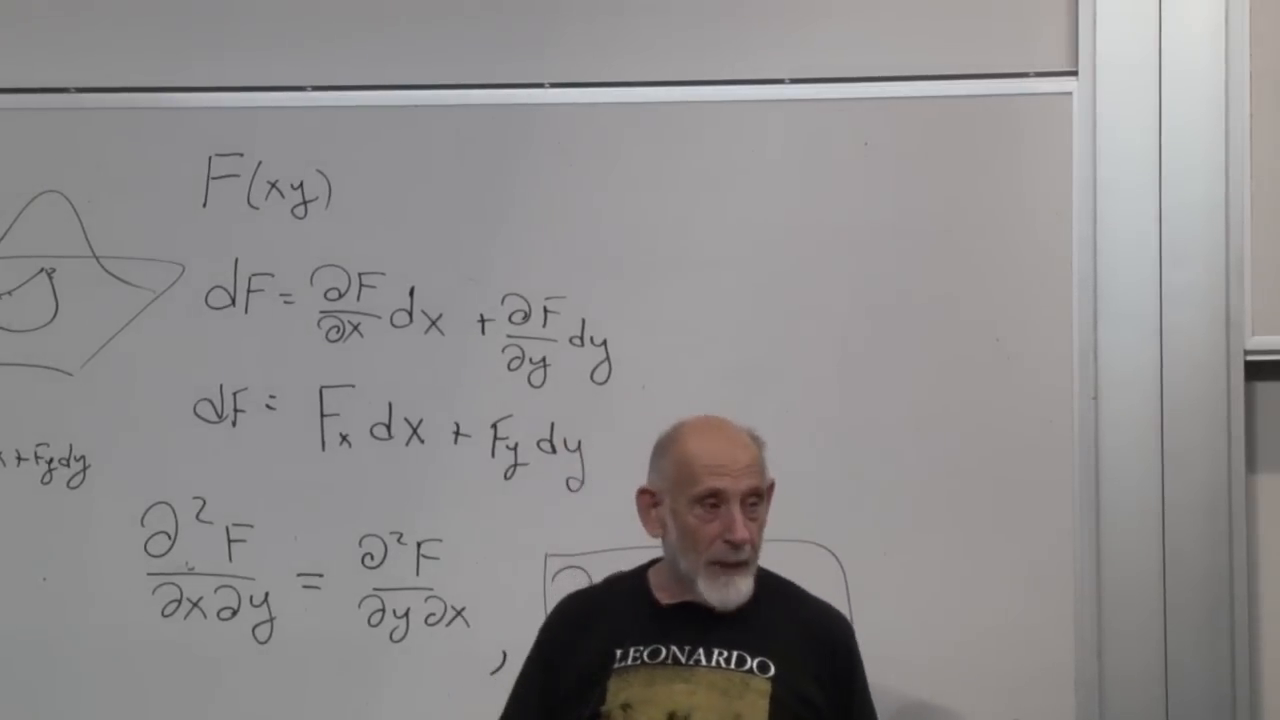
\includegraphics[width=0.90\textwidth]{lecture_06_figure_11.png}
\caption{高度作为标量函数、其微分，以及恰当性的混合偏导条件。}
\lectureframe{01:34:30}
\end{figure}

同一条件还有积分含义。若\(\omega=df\)，则
\begin{equation}
 \int_{\gamma:1\to2}\omega=f(2)-f(1)
 \label{eq:sm6-path-independent-integral}
\end{equation}
仅依赖于端点，而不依赖于路径\(\gamma\)。特别地，
\begin{equation}
 \oint_\gamma\omega=0
 \label{eq:sm6-closed-loop-zero}
\end{equation}
对每一条可收缩的闭合回路成立。

高度具有这一性质。沿平坦道路或翻越山丘在同两点之间行驶，高度的净变化相同。燃料消耗则不然。多山路线与平坦路线通常消耗不同的量，而一次闭合行程并不会恢复已燃烧的燃料。在扩展的状态描述中，剩余燃料量当然是一个定义明确的量，但它不是汽车位置\((x,y)\)单独的函数；它携带着路线的记忆。疲劳提供了同类的类比：下坡一般并不能消除上坡带来的疲劳。

\begin{classroomqa}
\audiencequestion{恰当性与保守力是同一概念吗？它与曲率有关吗？}
\lecturerresponse{旋度为零的力场是局部保守的，并允许存在势，因此这一语言密切相关。平行移动和曲率也将闭合回路的变化与局部几何数据联系起来，但那是一个更广泛的课题。这里只需要初等的陈述：零旋度意味着局部路径无关性，并带有通常关于区域的整体条件。
\lecturetimestamp{01:39:22--01:41:07}}
\end{classroomqa}

两个例子使这一检验具体化。首先取
\begin{equation}
 F_x=y,\qquad F_y=x.
 \label{eq:sm6-exact-example}
\end{equation}
两个交叉导数都等于\(1\)，确实
\begin{equation}
 \omega=y\,dx+x\,dy=d(xy).
 \label{eq:sm6-exact-example-potential}
\end{equation}
现在改变一个符号：
\begin{equation}
 F_x=y,\qquad F_y=-x.
 \label{eq:sm6-inexact-example}
\end{equation}
于是
\begin{equation}
 \frac{\partial F_x}{\partial y}=1,
 \qquad
 \frac{\partial F_y}{\partial x}=-1,
 \label{eq:sm6-inexact-cross-derivatives}
\end{equation}
因此不存在标量\(f(x,y)\)以这两个分量作为其梯度。

\begin{figure}[t]
\centering
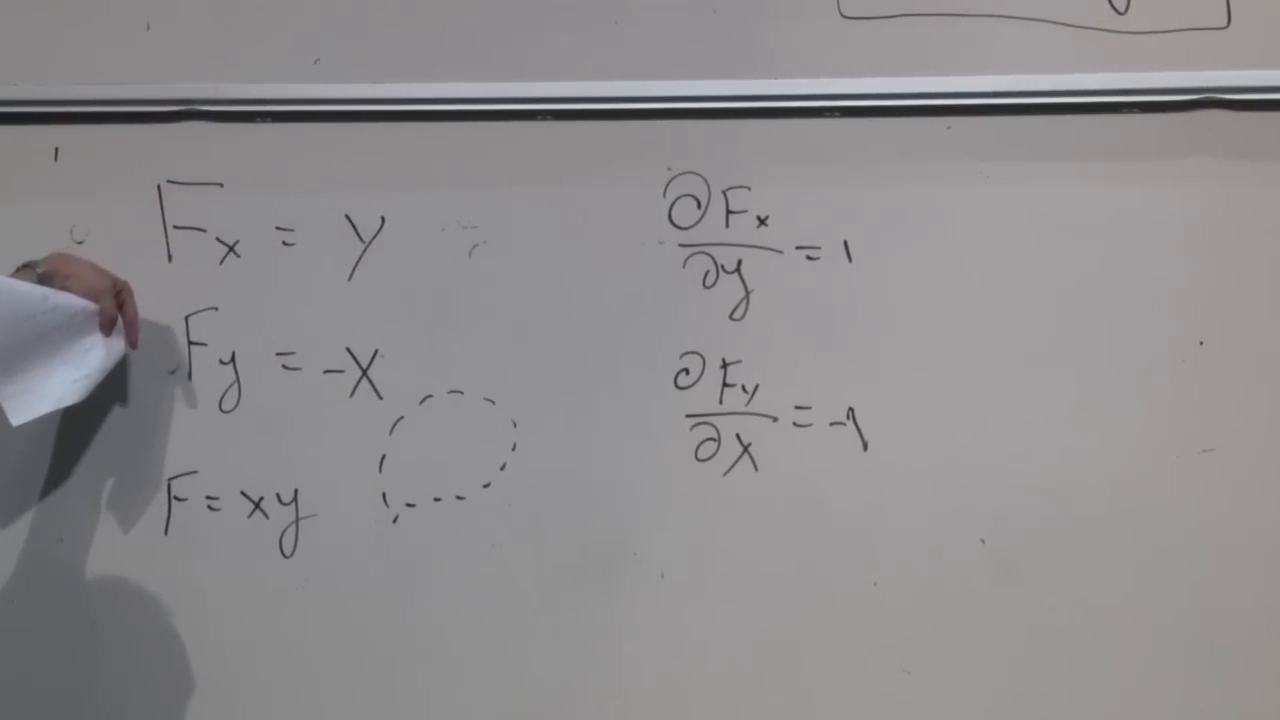
\includegraphics[width=0.90\textwidth]{lecture_06_figure_12.png}
\caption{一个由\(f=xy\)生成的恰当例子，以及一个交叉导数为\(1\)和\(-1\)的非恰当例子。}
\lectureframe{01:44:50}
\end{figure}

\section{热量与功不是态函数}

对于粒子数固定的简单可压缩系统，两个独立的平衡变量决定状态。我们可以使用\((T,V)\)、\((E,V)\)，或者，尤其对于基本关系而言自然地使用\((S,V)\)。因此
\begin{equation}
 E=E(S,V),
 \end{equation}
其恰当微分为
\begin{equation}
 dE=
 \left(\frac{\partial E}{\partial S}\right)_V dS+
 \left(\frac{\partial E}{\partial V}\right)_S dV
 =T\,dS-P\,dV.
 \label{eq:sm6-fundamental-relation}
\end{equation}

\begin{classroomqa}
\audiencequestion{绝热是指缓慢、绝热绝缘、可逆，还是等熵？}
\lecturerresponse{这一术语在不同语境中用法不同。对于此处考虑的平衡路径，变化是准静态且热绝缘的，因此是可逆且等熵的。仅仅绝缘的不可逆过程仍可产生熵，而量子绝热定理则强调参数的缓慢变化。
\lecturetimestamp{01:47:13--01:47:54}}
\end{classroomqa}

在熵固定时，膨胀使气体能量变化
\(-P\,dV\)。在体积固定时，可逆传热使其变化
\(T\,dS\)。因此，将下式写出是有用的：
\begin{equation}
 \begin{aligned}
 \delta W_{\mathrm{on}}&=-P\,dV,
 &\delta Q_{\mathrm{rev}}&=T\,dS,\\
 dE&=\delta Q_{\mathrm{rev}}+\delta W_{\mathrm{on}}.&&
 \end{aligned}
 \label{eq:sm6-first-law-increments}
\end{equation}
符号\(\delta\)而非\(d\)，预示着热和功是路径增量，而不是状态函数的微分。

\begin{figure}[t]
\centering
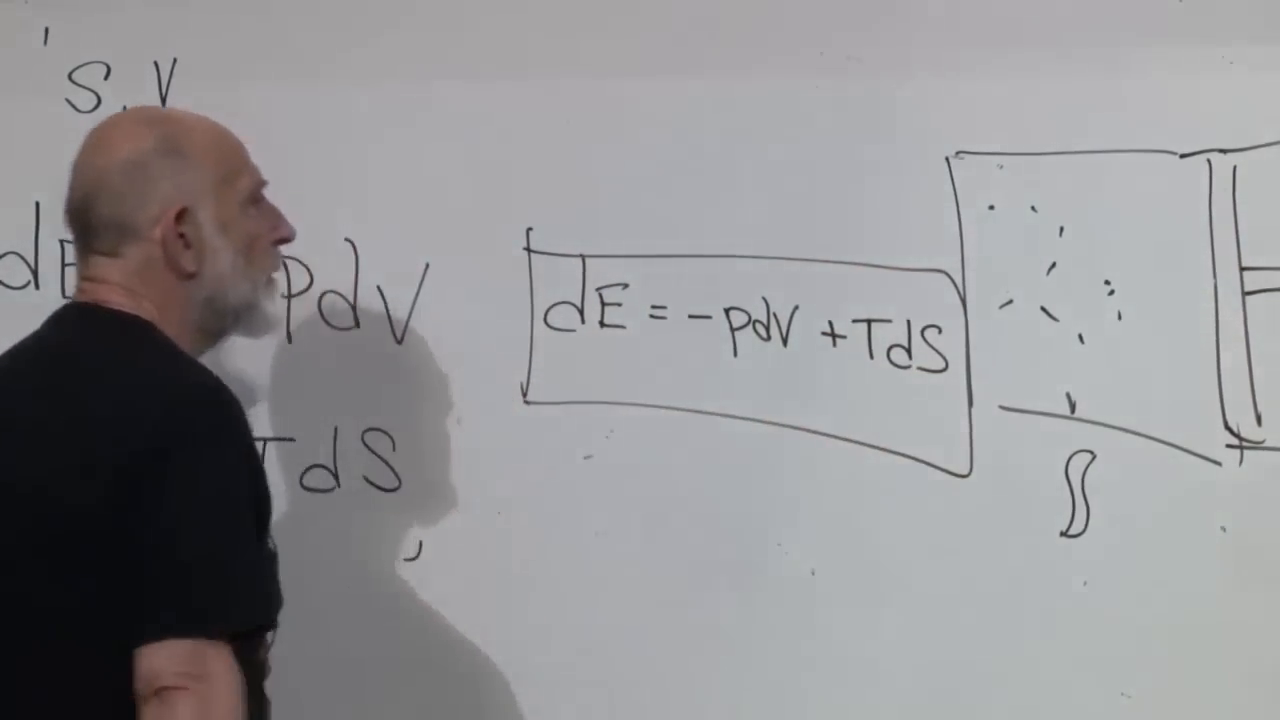
\includegraphics[width=0.90\textwidth]{lecture_06_figure_13.png}
\caption{活塞系统的第一定律：
\(dE=-P\,dV+T\,dS\)。}
\lectureframe{01:50:28}
\end{figure}

\begin{classroomqa}
\audiencequestion{\(-P\,dV\)表示对气体做的功还是气体做的功？}
\lecturerresponse{按照
\eqref{eq:sm6-first-law-increments}中的约定，它是对气体做的功。在膨胀过程中\(dV>0\)，气体对活塞做正功，因此对气体做的功为负，气体失去能量。这两种描述大小相等、方向相反。
\lecturetimestamp{01:51:23--01:52:27}}
\end{classroomqa}

等式\(\delta Q_{\mathrm{rev}}=T\,dS\)绝不能原封不动地推广到任意不可逆加热。一般而言，
\begin{equation}
 dS=\frac{\delta Q}{T_{\mathrm{boundary}}}+dS_{\mathrm{prod}},
 \qquad dS_{\mathrm{prod}}\ge 0.
 \label{eq:sm6-entropy-production}
\end{equation}
下面关于全微分的论证针对准静态平衡路径，对于这些路径，可逆关系是恰当的关系。

\begin{classroomqa}
\audiencequestion{在态空间论证中，是否假定所有路径都经过平衡态？}
\lecturerresponse{是的。这些操作进行得足够缓慢，使得\(P\)、\(T\)、\(E\)、\(S\)和\(V\)沿路径始终保持良好定义。热和功的路径依赖性并不要求系统被驱离平衡态很远。
\lecturetimestamp{01:54:30--01:54:39}}
\end{classroomqa}

要检验热是否为全微分，以\((E,V)\)为坐标并重新整理第一定律：
\begin{equation}
 \delta Q_{\mathrm{rev}}=dE+P(E,V)\,dV.
 \label{eq:sm6-heat-one-form}
\end{equation}
如果存在状态函数\(Q(E,V)\)满足\(dQ=\delta Q_{\mathrm{rev}}\)，则其偏导数必须为
\begin{equation}
 \left(\frac{\partial Q}{\partial E}\right)_V=1,
 \qquad
 \left(\frac{\partial Q}{\partial V}\right)_E=P.
 \label{eq:sm6-hypothetical-heat-derivatives}
\end{equation}
于是混合导数相等将要求
\begin{equation}
 \begin{aligned}
 \frac{\partial}{\partial V}
 \left(\frac{\partial Q}{\partial E}\right)_V
 &=\frac{\partial}{\partial E}
 \left(\frac{\partial Q}{\partial V}\right)_E,\\
 0&=\left(\frac{\partial P}{\partial E}\right)_V.
 \end{aligned}
 \label{eq:sm6-heat-exactness-requirement}
\end{equation}

\begin{classroomqa}
\audiencequestion{这与用于\(F_x\,dx+F_y\,dy\)的旋度检验完全相同吗？}
\lecturerresponse{是的。\(dE\)和\(dV\)的系数分别是\(1\)和
\(P(E,V)\)。它们的交叉导数分别是\(0\)和
\((\partial P/\partial E)_V\)。只有当这些导数一致时，热才是全微分。
\lecturetimestamp{01:54:39--01:54:52}}
\end{classroomqa}

\begin{figure}[t]
\centering
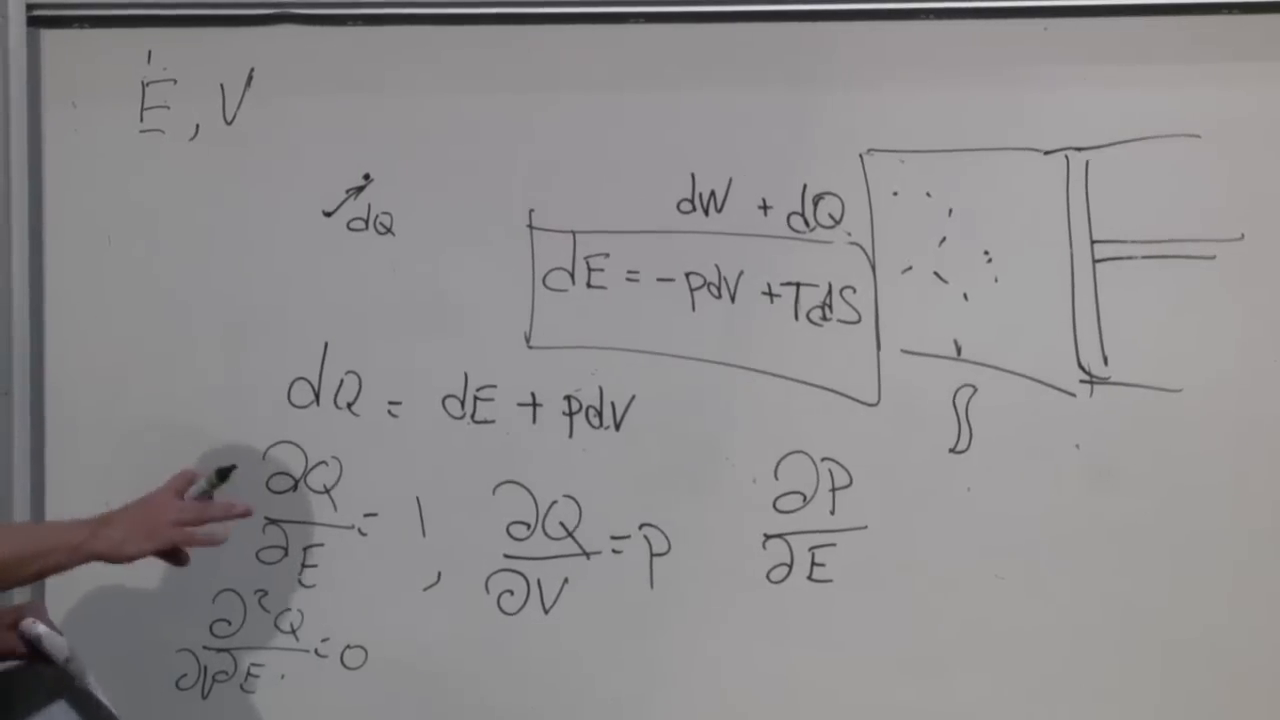
\includegraphics[width=0.90\textwidth]{lecture_06_figure_14.png}
\caption{热的一形式\(dE+P\,dV\)，以及若它是某个状态函数的微分则所需的混合导数。}
\lectureframe{01:58:10}
\end{figure}

这一要求从物理上就已经不可信：在体积固定时向气体添加能量通常会改变其压强。理想气体提供了一个直接的计算：
\begin{equation}
 PV=NT,
 \qquad
 E=\frac{3}{2}NT
 \quad\Longrightarrow\quad
 P=\frac{2E}{3V}.
 \label{eq:sm6-ideal-pressure-energy}
\end{equation}
因此
\begin{equation}
 \left(\frac{\partial P}{\partial E}\right)_V
 =\frac{2}{3V}\ne0.
 \label{eq:sm6-heat-curl-fails}
\end{equation}
旋度检验失败：\(\delta Q_{\mathrm{rev}}\)不是全微分。功的增量\(\delta W_{\mathrm{on}}=-P\,dV\)出于同样的原因也失败。

\begin{figure}[t]
\centering
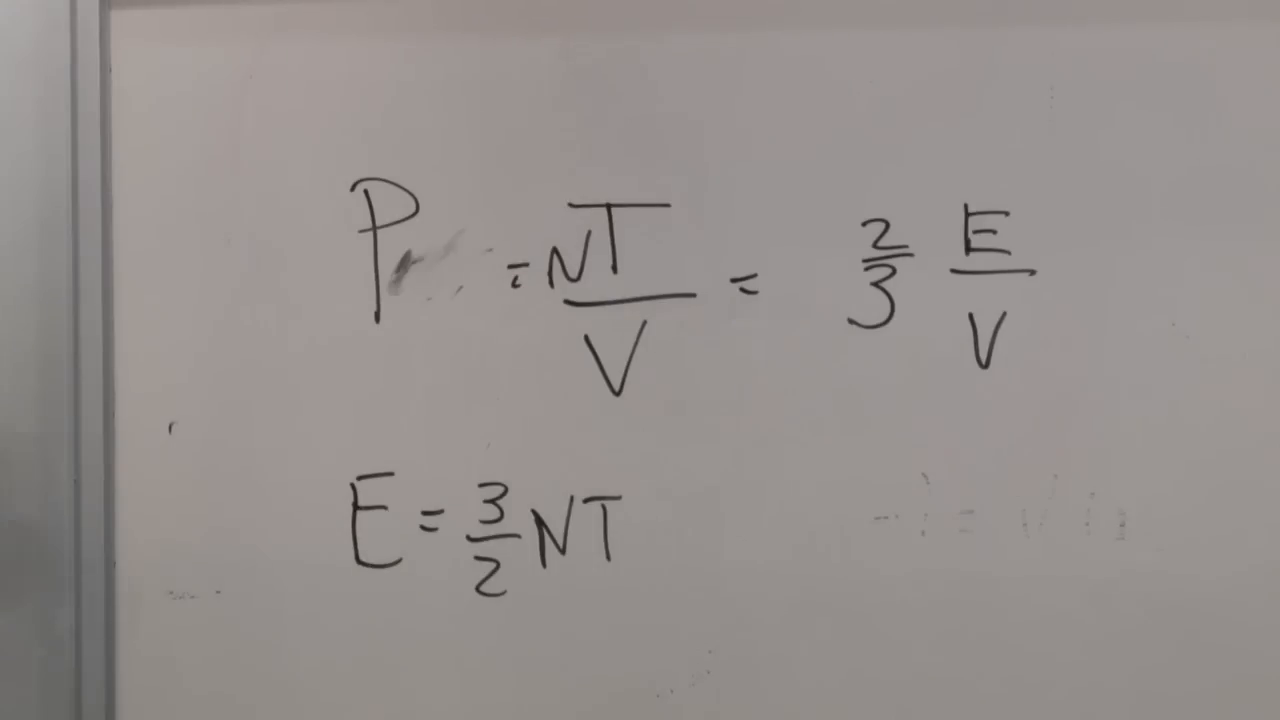
\includegraphics[width=0.90\textwidth]{lecture_06_figure_15.png}
\caption{将理想气体关系合并为
\(P=2E/(3V)\)。}
\lectureframe{02:00:00}
\end{figure}

\begin{figure}[H]
\centering
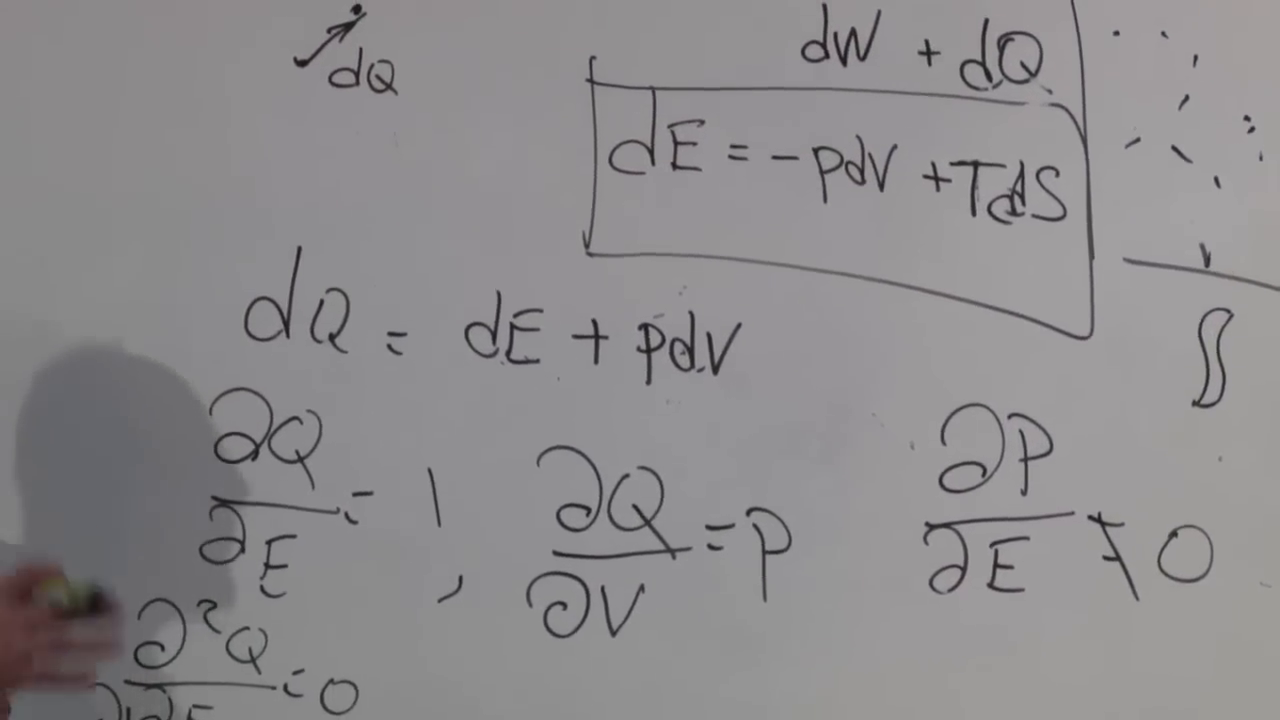
\includegraphics[width=0.90\textwidth]{lecture_06_figure_16.png}
\caption{完整的论证：因为
\((\partial P/\partial E)_V\ne0\)，热的一形式不可能是全微分。}
\lectureframe{02:00:35}
\end{figure}

对于封闭的平衡循环，
\begin{equation}
 \oint dE=0,
 \qquad
 \oint\delta Q_{\mathrm{rev}}
 =-\oint\delta W_{\mathrm{on}}.
 \label{eq:sm6-cycle-balance}
\end{equation}
系统回到相同的能量，但热和功不必分别消失。它们的值取决于在态空间中所走的路径。这就是为什么循环热机能够吸收热并输出净功，即使其工作物质回到初始热力学状态。

\begin{classroomqa}
\audiencequestion{这种路径依赖性与热机效率、滞后和记忆有关吗？}
\lecturerresponse{热机循环直接利用它：循环的热输入与净功输出相平衡，而状态函数\(E\)回到其初始值。滞后和记忆也涉及路径依赖性，尽管它们通常需要额外的内部变量或非平衡物理。目前的结论更为狭窄，并且已经对可逆平衡路径成立：热和功是转移量，而不是储存在热力学状态中的属性。
\lecturetimestamp{02:02:21--02:03:17}}
\end{classroomqa}

论证的两个部分现在汇合了。只有当其控制条件和平衡条件被指定后，测量才有意义。只有当其小参数和失效判据被指定后，近似才有意义。只有当其微分通过路径无关性检验后，热力学量才是状态函数。在每一种情形中，严谨的数学并不取代物理解释；它确切地告诉我们这种解释在何处是合理的。